%-----------------------------------------------------------------------------%
\addChapter{Lampiran 1 : Pattern Buatan Manual}
\chapter*{Lampiran 1 : Pattern Buatan Manual}
%-----------------------------------------------------------------------------%
Berikut adalah daftar \textit{pattern} yang dibentuk secara manual oleh anotator.
\begin{itemize}
  \item <hypernym> adalah kumpulan dari <hyponym>
  \item <hypernym> antara lain adalah <hyponym>, <hyponym>, dan <hyponym>
  \item <hypernym> dapat dibedakan menjadi <hyponym>
  \item <hypernym> lainnya, seperti <hyponym> dan <hyponym>
  \item <hypernym> seperti <hyponym>
  \item <hypernym> terdiri dari <hyponym>, <hyponym>, dan <hyponym>
  \item <hypernym> terdiri dari beberapa bagian, seperti <hyponym>, <hyponym>, dan <hyponym>
  \item <hypernym> terutama <hyponym> yang
  \item <hypernym>, khususnya <hyponym>, adalah
  \item <hypernym>, misalnya <hyponym>
  \item <hypernym>, misalnya <hyponym> dan <hyponym>
  \item <hypernym>, terutama <hyponym>, adalah
  \item <hyponym> adalah <hypernym>
  \item <hyponym> adalah <hypernym> dari
  \item <hyponym> adalah <hypernym> dengan
  \item <hyponym> adalah <hypernym> yang berhubungan dekat dengan <hyponym>
  \item <hyponym> adalah <hypernym> yang bersifat
  \item <hyponym> adalah bagian dari <hypernym> yang
  \item <hyponym> adalah salah satu <hypernym>
  \item <hyponym> adalah sebuah <hypernym> yang
  \item <hyponym> adalah sejenis <hypernym> dengan
  \item <hyponym> adalah suatu <hypernym>
  \item <hyponym> atau <hyponym> adalah suatu jenis <hypernym> yang
  \item <hyponym> berarti <hypernym>
  \item <hyponym> dan <hyponym> dianggap sebagai <hypernym>
  \item <hyponym> dan <hyponym> merupakan <hypernym> yang
  \item <hyponym> dan berbagai <hyponym> lainnya adalah <hypernym> yang
  \item <hyponym> dan sejumlah <hyponym> lainnya termasuk ke dalam kategori <hypernym>
  \item <hyponym> dapat digolongkan ke dalam <hypernym>
  \item <hyponym> dapat dimasukkan ke dalam kategori <hypernym> dan <hypernym>
  \item <hyponym> dianggap sebagai <hypernym> karena
  \item <hyponym> dikenal juga sebagai <hypernym>
  \item <hyponym> disebut sebagai <hypernym> yang
  \item <hyponym> ialah <hypernym>
  \item <hyponym> menjadi <hypernym> apabila
  \item <hyponym> menjadi <hypernym> yang
  \item <hyponym> menjadi salah satu bagian dari <hypernym> karena
  \item <hyponym> merujuk pada <hypernym>
  \item <hyponym> merujuk pada <hypernym> yang
  \item <hyponym> merupakan <hypernym>
  \item <hyponym> merupakan <hypernym> yang
  \item <hyponym> merupakan suatu <hypernym> yang
  \item <hyponym> secara khusus menjadi sebutan bagi <hypernym> yang
  \item <hyponym> termasuk <hypernym> yang
  \item <hyponym> termasuk ke dalam <hypernym> yang
  \item <hyponym> termasuk ke dalam kategori <hypernym>
  \item <hyponym> termasuk ke dalam salah satu <hypernym> yang
  \item <hyponym> tersebut merupakan <hypernym>
  \item Beberapa <hypernym> seperti <hyponym>
  \item Beberapa contoh <hypernym> lainnya adalah <hyponym>
  \item Beberapa jenis dari <hypernym> adalah <hyponym> dan <hyponym>
  \item Berbagai <hypernym> seperti <hyponym>
  \item Contoh dari <hypernym> adalah <hyponym>
  \item Contoh dari <hypernym>, yaitu <hyponym>, <hyponym>, dan <hyponym>
  \item Istilah umum dari <hyponym> adalah <hypernym>
  \item Jenis <hypernym> yang paling banyak dikenal adalah <hyponym>
  \item Jenis-jenis <hypernym> antara lain <hyponym> dan <hyponym>
  \item Salah satu <hypernym> adalah <hyponym>
  \item Salah satu <hypernym> yang mirip dengan <hyponym> adalah <hyponym>
  \item Salah satu contoh dari <hypernym> adalah <hyponym>
  \item Sebagai salah satu <hypernym>, <hyponym>
  \item Sebagai sebuah <hypernym>, <hyponym> merupakan
  \item Secara umum, <hyponym> merupakan <hypernym> yang dapat
  \item Selain <hyponym>, <hyponym> juga menjadi <hypernym> yang
  \item Terdapat banyak <hypernym>, seperti <hyponym>
  \item Terdapat beberapa contoh <hypernnym>, di antaranya <hyponym>, <hyponym>, dan <hyponym>
  \item Walaupun <hyponym> adalah <hypernym>, tetapi 
\end{itemize}

%-----------------------------------------------------------------------------%
\addChapter{Lampiran 2 : Panduan Pembuatan dan Anotasi Pattern}
% \chapter*{Lampiran 2 : Panduan Pembuatan danaa Anotasi Pattern}
%-----------------------------------------------------------------------------%
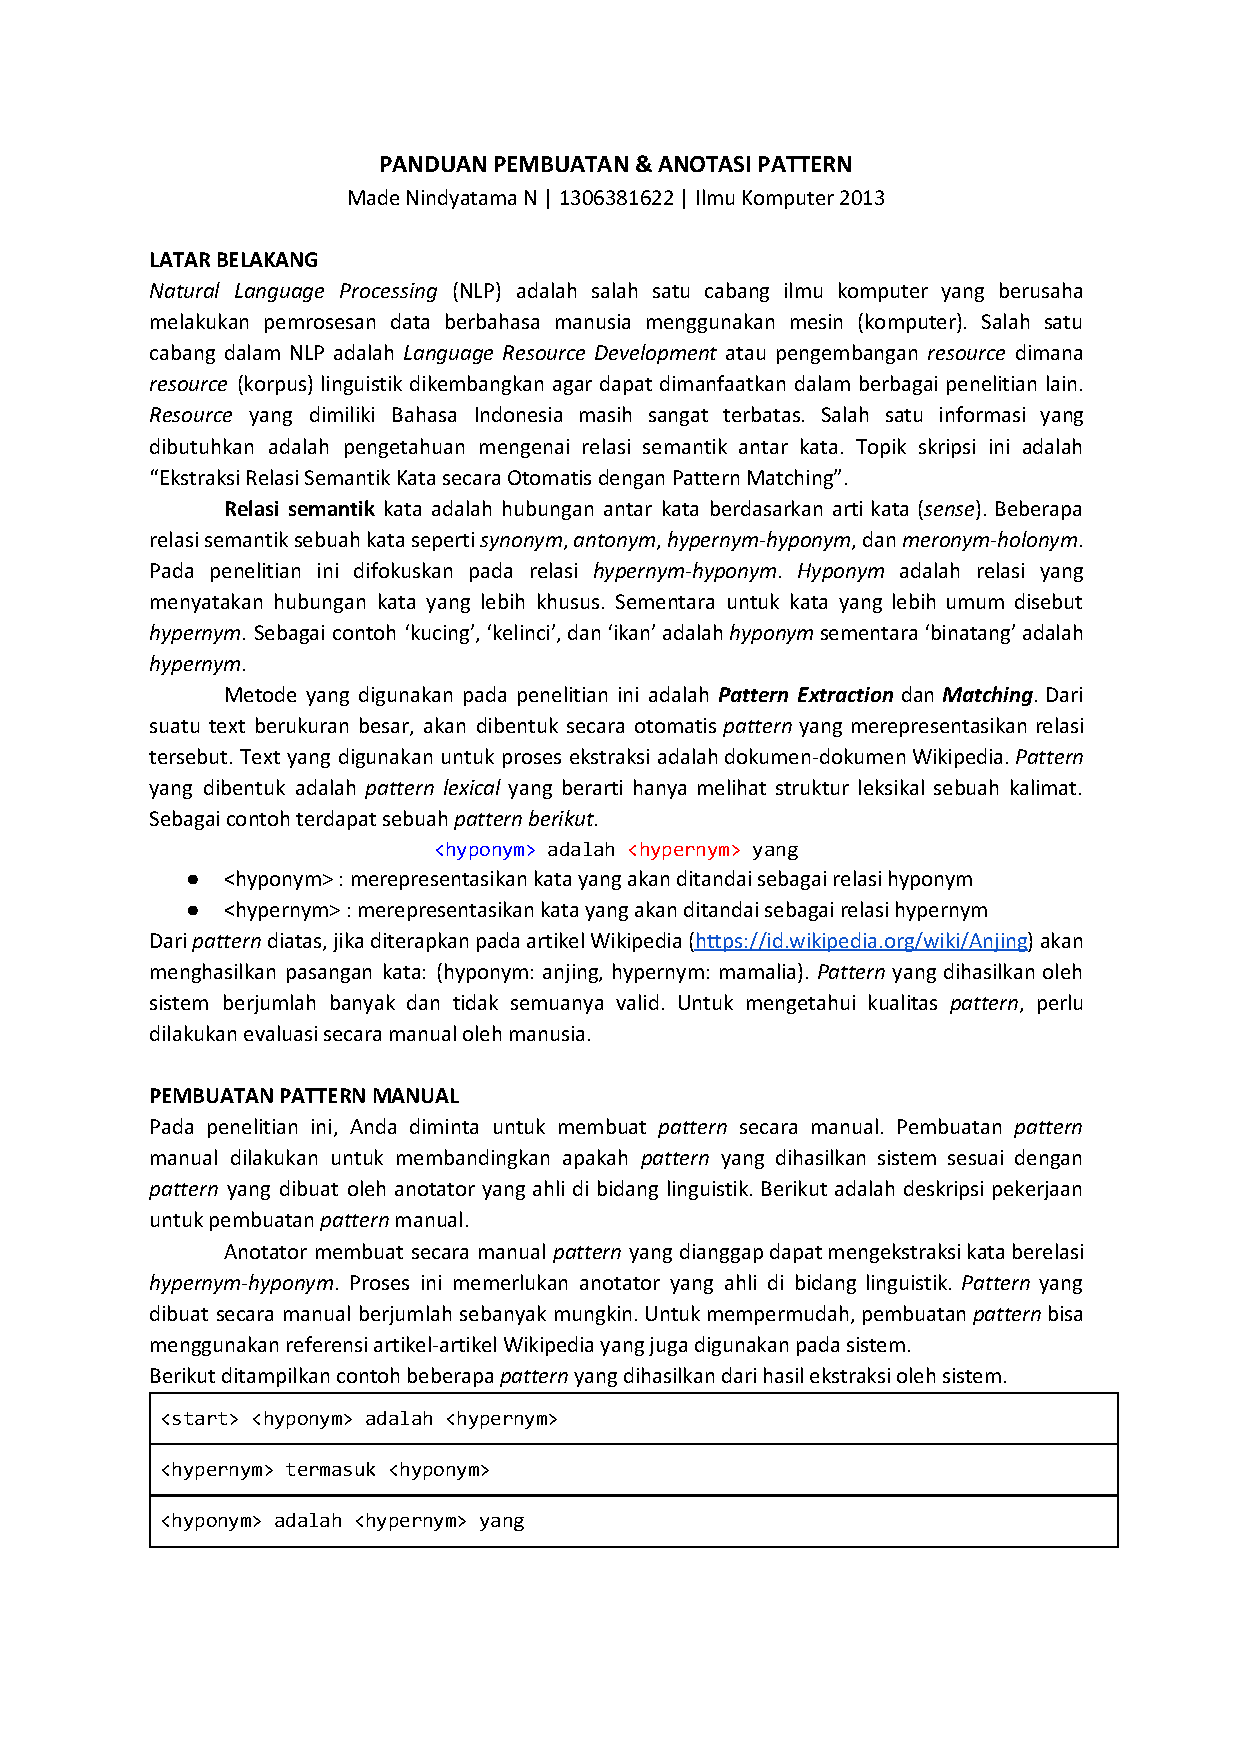
\includepdf[pages={1}]{PanduanPembuatanAnotasiPattern.pdf}
\includepdf[pages={2}]{PanduanPembuatanAnotasiPattern.pdf}

%-----------------------------------------------------------------------------%
\addChapter{Lampiran 3 : Panduan Anotasi Pair}
%-----------------------------------------------------------------------------%
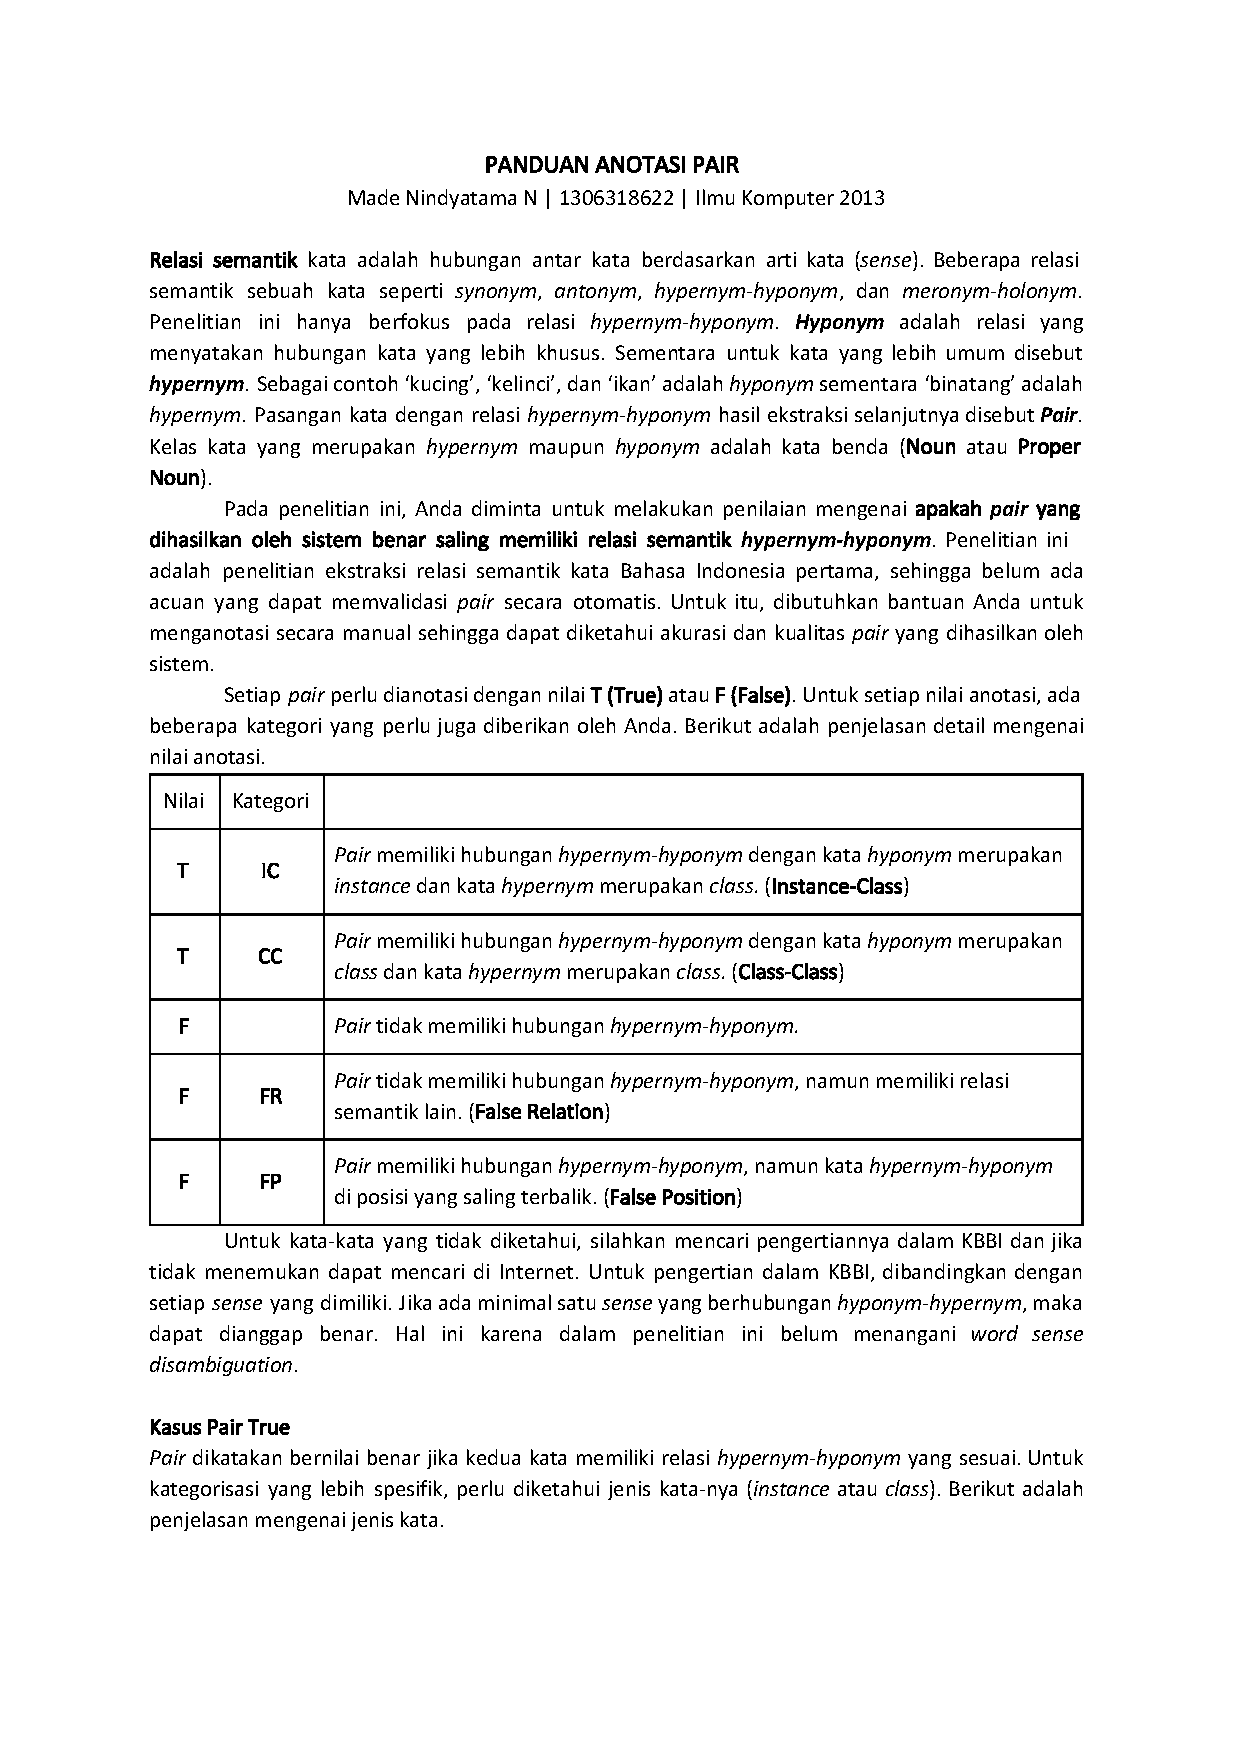
\includepdf[pages={1}]{PanduanAnotasiPair.pdf}
\includepdf[pages={2}]{PanduanAnotasiPair.pdf}
\includepdf[pages={3}]{PanduanAnotasiPair.pdf}

% \section*{\code{admin\_useraddmaster}} \label{cha:lampir-admin}
% Skrip ini diletakkan pada direktori \co{/usr/sesuatu} dan hanya dapat dieksekusi oleh \f{root}. Skrip ini berguna untuk menambahkan pengguna baru sesuai dengan konfigurasi baru yang telah ditetapkan.
% \begin{lstlisting}[style=L,caption={Skrip menambahkan pengguna baru},label={lst:adduser}]
% #!/bin/csh -f
% blah blah blah
% blah blah blah
% blah blah blah
% blah blah blah
% blah blah blah
% \end{lstlisting}

% \section*{\code{getuser.cron}} \label{cha:lampir-cronadmin}
% Penjelasan skrip disini
% \begin{lstlisting}[style=L,caption={\f{Cronjob} menambahkan pengguna baru},label={lst:cronadduser}]
% #!/bin/bash
% # Change these two lines to localize to your system:
% # Adapted from /usr/local/sbin/admin_useradd

% cat /dev/null > $userlist
% for (( i=0; i<${#listemailto[@]}; i++ ))
% do
%         uname=${listusername[$i]}
%         mailto=${listemailto[$i]}

%         echo "User $uname created, please use torqace wisely." | mail -s "Torqace user registration" $mailto
% done

% \end{lstlisting}
% 
% %-----------------------------------------------------------------------------%
% \addChapter{Lampiran 2 : Berkas Konfigurasi}
% \chapter*{Lampiran 2 : Berkas Konfigurasi}
% %-----------------------------------------------------------------------------%
% \section*{compute.xml}
% \begin{lstlisting}[caption={Berkas \co{compute.xml}},label={lst:excomp},language=XML]
% <?xml version="1.0" standalone="no"?>
% <kickstart>
% <description>
% 	Compute node XML file
% </description>
% </kickstart> 
% \end{lstlisting}

% %-----------------------------------------------------------------------------%
% \addChapter{Lampiran 8 : UAT dan Kuesioner}
% %-----------------------------------------------------------------------------%
% \begin{landscape}
% \chapter*{Lampiran 8 : UAT dan Kuesioner}
% \begin{longtable}{|c|p{7cm}|p{2.5cm}|p{3.5cm}|p{3.3cm}|p{1.8cm}|}
% \caption{Tabel UAT dan Kuesioner} \label{tab:uattbl}\\
% \hline
% No. & \multicolumn{1}{c|}{Langkah Penggunaan} & Fitur Berjalan & Tingkat Kemudahan (1-5) & Tingkat Kepuasan (1-5) & Saran / Komentar \\ 
% \cline{3-5} & & Berhasil /Tidak & 1:Sangat sulit ; \hspace{100pt} 5:sangat mudah & 1 : Sangat kecewa ; 5 : sangat puas &  \\ \hline
% \multicolumn{ 6}{|>{\columncolor{headertbl}}c|}{Use Case : Login} \\ \hline
% 1.1 & Pengguna berada pada halaman depan torqace &  &  &  &  \\ \hline
% 1.2 & Pengguna memasukkan username dan password pada field yang telah disediakan.Kemudian menekan tombol 'login' &  &  &  &  \\ \hline
% 1.3 & Apabila Sukses, maka pengguna masuk ke dalam sistem dan dihadapkan pada menu utama &  &  &  &  \\ \hline
% \multicolumn{ 6}{|>{\columncolor{headertbl}}c|}{Use Case : Register} \\ \hline
% 2.1 & Pengguna berada pada halaman registrasi pengguna torqace &  &  &  &  \\ \hline
% 2.2 & Pengguna memasukkan username,password, dan email pada field yang telah disediakan. Kemudian menekan tombol 'submit' &  &  &  &  \\ \hline
% 2.3 & Sistem akan mengonfirmasi masukan, dan akan mengirimkan email untuk memberitahu pengguna apabila proses pendaftaran telah selesai &  &  &  &  \\ \hline
% \multicolumn{ 6}{|>{\columncolor{headertbl}}c|}{Use Case : Logout} \\ \hline
% 3.1 & Pengguna memilih menu untuk melakukan logout &  &  &  &  \\ \hline
% 3.2 & Sistem akan mengeluarkan pengguna, dan pengguna tidak dapat menggunakan fitur-fitur utama aplikasi &  &  &  &  \\ \hline
% \multicolumn{ 6}{|>{\columncolor{headertbl}}c|}{Use Case : Upload Job Sederhana} \\ \hline
% 4.1 & Pengguna memilih menu upload file/project pada menu utama &  &  &  &  \\ \hline
% 4.2 & Pengguna memilih pilihan 'single file' pada tipe project &  &  &  &  \\ \hline
% 4.3 & Pengguna memilih berkas yang akan diunggah, mengisi label, dan menentukan apakah akan menimpa project sebelumnya dengan nama yang sama atau tidak &  &  &  &  \\ \hline
% 4.4 & Pengguna menekan tombol 'submit' dan mengonfirmasi  &  &  &  &  \\ \hline
% 4.5 & Sistem akan menampilkan informasi terkait berkas yang diupload &  &  &  &  \\ \hline
% \multicolumn{ 6}{|>{\columncolor{headertbl}}c|}{Use Case : Upload Job Compressed} \\ \hline
% 5.1 & Pengguna memilih menu upload file/project pada menu utama &  &  &  &  \\ \hline
% 5.2 & Pengguna memilih pilihan 'compressed files' pada tipe project &  &  &  &  \\ \hline
% 5.3 & Pengguna memilih arsip yang akan diunggah, mengisi label, menentukan akan melakukan make atau tidak dan menentukan apakah akan menimpa project sebelumnya dengan nama yang sama atau tidak &  &  &  &  \\ \hline
% 5.4 & Pengguna menekan tombol 'submit' dan mengonfirmasi  &  &  &  &  \\ \hline
% 5.5 & Sistem akan menampilkan informasi terkait berkas yang diupload dan diekstrak. Keluaran make juga akan ditampilkan bila dipilih &  &  &  &  \\ \hline
% \multicolumn{ 6}{|>{\columncolor{headertbl}}c|}{Use Case : Upload Array Job} \\ \hline
% 6.1 & Pengguna memilih menu upload file/project pada menu utama &  &  &  &  \\ \hline
% 6.2 & Pengguna memilih pilihan 'array' pada tipe project &  &  &  &  \\ \hline
% 6.3 & Pengguna memilih arsip-arsip yang akan diunggah, mengisi label, menentukan akan melakukan make atau tidak dan menentukan apakah akan menimpa project sebelumnya dengan nama yang sama atau tidak &  &  &  &  \\ \hline
% 6.4 & Pengguna menekan tombol 'submit' dan mengonfirmasi  &  &  &  &  \\ \hline
% 6.5 & Sistem akan menampilkan informasi terkait berkas yang diupload dan diekstrak. Keluaran make juga akan ditampilkan bila dipilih &  &  &  &  \\ \hline
% \multicolumn{ 6}{|>{\columncolor{headertbl}}c|}{Use Case : Melihat antrian pada queue} \\ \hline
% 7.1 & Pengguna memilih menu  queue status pada menu utama &  &  &  &  \\ \hline
% 7.2 & Pengguna berada pada halaman yang berisi informasi queue &  &  &  &  \\ \hline
% \multicolumn{ 6}{|>{\columncolor{headertbl}}c|}{Use Case : Melihat detil antrian} \\ \hline
% 8.1 & Dari halaman status queue, pengguna memilih job tertentu &  &  &  &  \\ \hline
% 8.2 & Informasi mengenai detil job tersebut ditampilkan dalam bentuk tabel &  &  &  &  \\ \hline
% 8.2.1 & Apabila job tersebut bukan milik pengguna, maka sistem akan melarang pengguna melihat informasi detil suatu job &  &  &  &  \\ \hline
% \multicolumn{ 6}{|>{\columncolor{headertbl}}c|}{Use Case : Membuat script job} \\ \hline
% 9.1 & Pengguna memilih untuk melakukan 'generate script' baik dari laporan upload berkas, atau dari penjelajahan direktori &  &  &  &  \\ \hline
% 9.2 & Pengguna mengisi nama job, parameter job, dan script yang akan dijalankan.  &  &  &  &  \\ \hline
% 9.3 & Pengguna mengonfirmasi konfirmasi submit job &  &  &  &  \\ \hline
% 9.4 & Pengguna dapat melihat informasi script secara keseluruhan dan pesan apakah terjadi kegagalan atau tidak, serta id job yang diberikan &  &  &  &  \\ \hline
% \multicolumn{ 6}{|>{\columncolor{headertbl}}c|}{Use Case : Load spesifikasi job lain} \\ \hline
% 10.1 & Pengguna berada pada halaman untuk membuat script &  &  &  &  \\ \hline
% 10.2 & Pengguna memilih 'Load a Previous Job' &  &  &  &  \\ \hline
% 10.3 & Pengguna memilih job mana yang akan dimuat dan menekan tombol 'Load' &  &  &  &  \\ \hline
% 10.4 & Pengguna kembali ke halaman pembuatan script dengan spesifikasi job sebelumnya &  &  &  &  \\ \hline
% \multicolumn{ 6}{|>{\columncolor{headertbl}}c|}{Use Case : Menjelajah Direktori} \\ \hline
% 11.1 & Pengguna memilih menu  'View File/Project'  pada menu utama &  &  &  &  \\ \hline
% 11.2 & Pengguna dapat melakukan navigasi untuk masuk ke dalam direktori tertentu, atau kembali ke direktori diatasnya, dan dapat melihat terdapat berkas apa saja dalam direktori &  &  &  &  \\ \hline
% \multicolumn{ 6}{|>{\columncolor{headertbl}}c|}{Use Case : Menghapus Berkas/Direktori} \\ \hline
% 12.1 & Pengguna berada pada halaman penjelajahan direktori &  &  &  &  \\ \hline
% 12.2 & Pengguna memilih pilihan untuk menghapus berkas/direktori di samping item yang akan dihapus &  &  &  &  \\ \hline
% 12.3 & Pengguna mengonfirmasi konfirmasi penghapusan &  &  &  &  \\ \hline
% \multicolumn{ 6}{|>{\columncolor{headertbl}}c|}{Use Case : Mengunduh Berkas/Direktori} \\ \hline
% 13.1 & Pengguna berada pada halaman penjelajahan direktori &  &  &  &  \\ \hline
% 13.2 & Pengguna memilih pilihan untuk mengunduh berkas/direktori di samping item yang akan dihapus &  &  &  &  \\ \hline
% \multicolumn{ 6}{|>{\columncolor{headertbl}}c|}{Use Case : Melihat Berkas} \\ \hline
% 14.1 & Pengguna berada pada halaman penjelajahan direktori &  &  &  &  \\ \hline
% 14.2 & Pengguna memilih berkas yang berupa berkas teks &  &  &  &  \\ \hline
% 14.3 & Sistem akan menampilkan konten dari berkas tersebut &  &  &  &  \\ \hline
% \end{longtable}
% \end{landscape}
